% Supplementary Figure S1 -- static-code architecture of Shopify's Web Pixels Manager (WPM).
% Final printed size: 190 mm x 90 mm (revised after review: no title baked into the figure; the caption carries it;
% code in Courier New at 7 pt; arrows as text glyphs, no math fonts). Every element comes from ../../notes/mechanism.md sections 2.1-2.5
% (static reading of wpm_manager_modern.js, build hash c8540278..., 2026-09-25) and from
% ../../crawl/CRAWL_NOTES.md section 5 (navigator overwrite inside STRICT workers).
% Encoding (FIGURE_PLAN.md): light grey strip = main thread; 45-degree hatch = Shopify sandbox.
% The accent red is deliberately NOT used: this is an architecture diagram, not a failure.
\documentclass[tikz,border=2pt]{standalone}
% schematic_style.tex -- shared style for every TikZ schematic panel (Fig 1a, 2a-2d).
% Binding source: ../../FIGURE_PLAN.md (style guide). Change colours here only.
% one sans face in BOTH engines (matplotlib panels use Arial too); Courier New for code (review: typography)
\usepackage{fontspec}\setmainfont{Arial}\setsansfont{Arial}\setmonofont{Courier New}
\renewcommand{\familydefault}{\sfdefault}
\usepackage{xcolor}
\usetikzlibrary{arrows.meta,calc,patterns.meta,shapes.geometric,positioning}

% ---- fixed vendor colours (FIGURE_PLAN.md, validated categorical order) ----
\definecolor{vGoogle}{HTML}{2A78D6}
\definecolor{vTikTok}{HTML}{EB6834}
\definecolor{vMeta}{HTML}{1BAF7A}
\definecolor{vPinterest}{HTML}{EDA100}
\definecolor{vSnap}{HTML}{E87BA4}
\definecolor{vMicrosoft}{HTML}{008300}
\definecolor{vOther}{HTML}{4A3AA7}
% ---- neutrals, arms (shape + grey, never hue), accent ----
\definecolor{ink}{HTML}{0B0B0B}      % text; Default arm
\definecolor{greyD}{HTML}{52514E}    % box outlines; Decline + Repeat arms
\definecolor{greyM}{HTML}{8A8984}    % sandbox hatch; GPC arm; secondary text
\definecolor{greyL}{HTML}{DEDDD9}    % main-thread origin (solid light grey)
\definecolor{greyXL}{HTML}{F3F2EF}   % faint container fill
\definecolor{accent}{HTML}{D03B3B}   % ONLY meaning: consent failed / blind spot
\colorlet{tbdgrey}{greyM}

% ---- sizes: 7 pt body, 10 pt bold panel letter ----
\newcommand{\fsBody}{\fontsize{7}{8.2}\selectfont}
\newcommand{\fsLetter}{\fontsize{10}{12}\selectfont\bfseries}
\newcommand{\fsTitle}{\fontsize{8}{9.6}\selectfont\bfseries}   % panel titles: 8 pt bold, as in the matplotlib panels (review FIG-20)

\tikzset{
  x=1mm, y=1mm,
  every picture/.style={line width=0.4pt},
  every node/.style={font=\fsBody, text=ink, inner sep=0.6mm},
  % arrows
  arr/.style={-{Stealth[length=1.5mm,width=1.1mm]}, draw=ink, line width=0.45pt},
  arrg/.style={-{Stealth[length=1.5mm,width=1.1mm]}, draw=greyD, line width=0.45pt},
  % boxes
  box/.style={draw=greyD, fill=white, rounded corners=0.7mm, line width=0.4pt},
  mainthread/.style={fill=greyL},
  sandbox/.style={pattern={Lines[angle=45,distance=1.25pt,line width=0.35pt]}, pattern color=greyM},
  % text helpers
  lbl/.style={align=left, anchor=north west, inner sep=0pt},
  lblc/.style={align=center, inner sep=0pt},
  note/.style={align=left, inner sep=0pt, text=greyD},
  panelletter/.style={font=\fsLetter, anchor=north west, inner sep=0pt},
  % arm markers (FIGURE_PLAN: Default filled circle #0b0b0b; Decline open square #52514e;
  % GPC filled triangle #8a8984; Repeat/validation open diamond #52514e)
  mDefault/.style={circle, fill=ink, draw=ink, inner sep=0pt, minimum size=2.1mm},
  mDecline/.style={rectangle, fill=white, draw=greyD, line width=0.7pt, inner sep=0pt, minimum size=1.85mm},
  mGPC/.style={regular polygon, regular polygon sides=3, fill=greyM, draw=greyM, inner sep=0pt, minimum size=2.7mm},
  mRepeat/.style={diamond, fill=white, draw=greyD, line width=0.7pt, inner sep=0pt, minimum size=2.4mm},
}

% vendor chip: \chip{vTikTok}  (small filled square; identity is always also named in text)
\newcommand{\chip}[1]{\tikz[baseline=-0.1mm]\fill[#1] (0,0) rectangle (1.7mm,1.7mm);}
% origin swatches for legends, same encoding as the data figures (3c)
\newcommand{\swMain}{\tikz[baseline=-0.1mm]\draw[greyD,fill=greyL,line width=0.3pt] (0,0) rectangle (3.2mm,1.9mm);}
\newcommand{\swSand}{\tikz[baseline=-0.1mm]\draw[greyD,line width=0.3pt,pattern={Lines[angle=45,distance=1.25pt,line width=0.35pt]},pattern color=greyM] (0,0) rectangle (3.2mm,1.9mm);}
% inline arm markers for text
\newcommand{\mkDefault}{\tikz[baseline=-0.75mm]\node[mDefault]{};}
\newcommand{\mkDecline}{\tikz[baseline=-0.75mm]\node[mDecline]{};}
\newcommand{\mkGPC}{\tikz[baseline=-0.95mm]\node[mGPC]{};}
\newcommand{\mkRepeat}{\tikz[baseline=-0.75mm]\node[mRepeat]{};}
\newcommand{\blindstar}{\tikz[baseline=-0.35mm]\node[star,star points=5,star point ratio=2.3,fill=accent,inner sep=0pt,minimum size=2.3mm]{};}

% Exact final size: standalone adds a 2pt border on every side, so the drawn
% bounding box is (W - 4pt) x (H - 4pt) and the PDF is exactly W x H.
\newcommand{\panelsize}[2]{\path[use as bounding box] (0,0) rectangle ($(#1,#2)-(4pt,4pt)$);}
\newcommand{\panelletter}[2]{\node[panelletter] at ($(0,#2)-(0,4pt)$) {#1};}

\newcommand{\obox}[5]{%
  \draw[box] (#1,#2) rectangle (#3,#4);
  \begin{scope}\clip[rounded corners=0.7mm] (#1,#2) rectangle (#3,#4);
    \fill[#5] (#1,#2) rectangle (#1+2.2,#4);\end{scope}
  \draw[greyD, rounded corners=0.7mm] (#1,#2) rectangle (#3,#4);}
\newcommand{\mono}[1]{{\fontsize{7}{8}\selectfont\ttfamily #1}}
\begin{document}
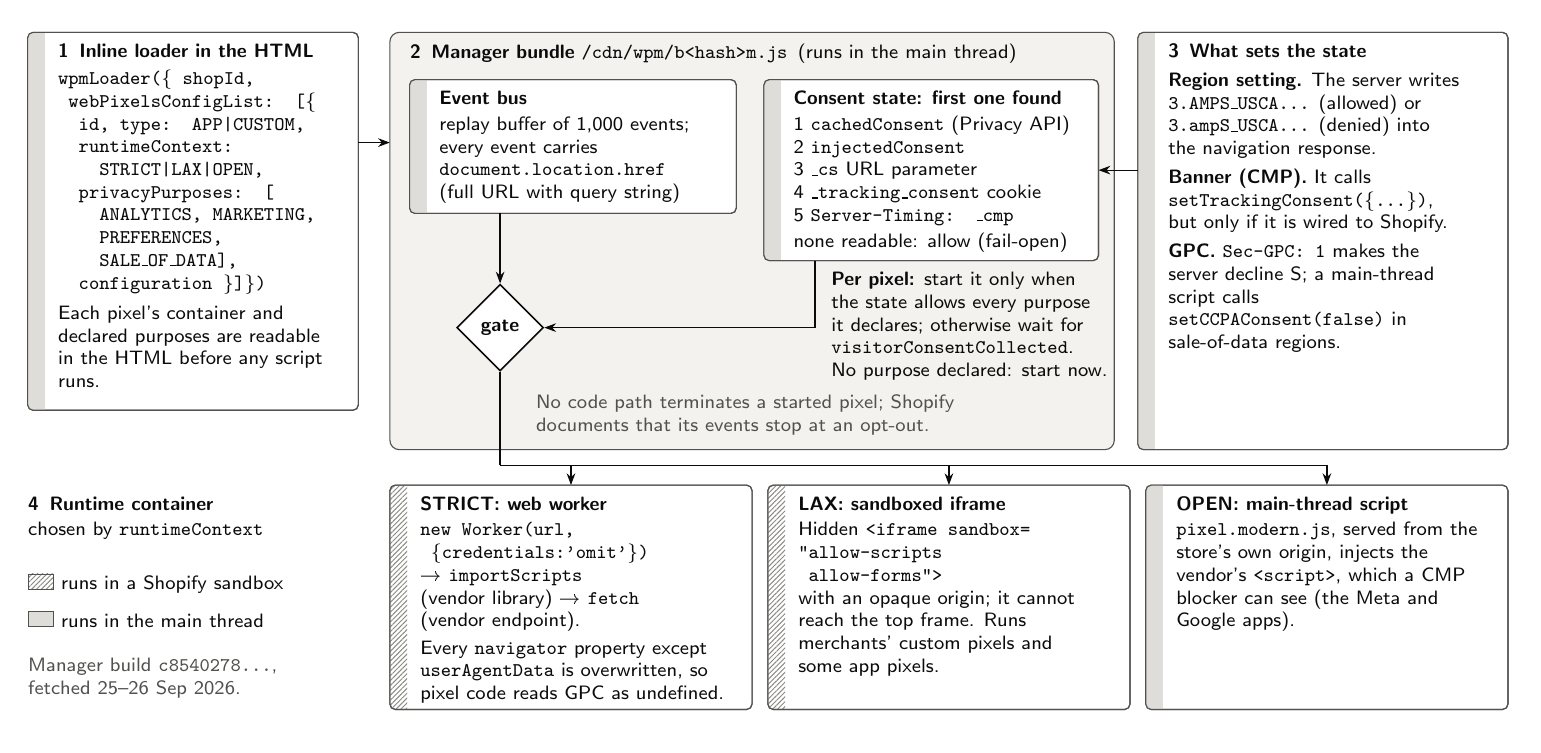
\begin{tikzpicture}
\def\W{190}\def\H{90}
\panelsize{\W}{\H}

% ---------------------------------------------------------------- 1. inline configuration
\obox{0}{40}{42}{88}{mainthread}
\node[lbl] at (3.8,86.6) {\textbf{1\enspace Inline loader in the HTML}\\[0.6mm]
  \mono{wpmLoader(\{ shopId,}\\
  \mono{\ webPixelsConfigList: [\{}\\
  \mono{\ \ id, type: APP|CUSTOM,}\\
  \mono{\ \ runtimeContext:}\\
  \mono{\ \ \ \ STRICT|LAX|OPEN,}\\
  \mono{\ \ privacyPurposes: [}\\
  \mono{\ \ \ \ ANALYTICS, MARKETING,}\\
  \mono{\ \ \ \ PREFERENCES,}\\
  \mono{\ \ \ \ SALE\_OF\_DATA],}\\
  \mono{\ \ configuration \}]\})}\\[1mm]
  Each pixel's container and\\ declared purposes are readable\\ in the HTML before any script\\ runs.};
\draw[arr] (42,74) -- (46,74);

% ---------------------------------------------------------------- 2. manager bundle (main thread)
\draw[draw=greyD, fill=greyXL, rounded corners=1.2mm] (46,35) rectangle (138,88);
\node[lbl] at (48.5,86.6) {\textbf{2\enspace Manager bundle} \mono{/cdn/wpm/b<hash>m.js}\enspace(runs in the main thread)};
% event bus
\obox{48.5}{65}{90}{82}{mainthread}
\node[lbl] at (52.2,80.6) {\textbf{Event bus}\\[0.4mm] replay buffer of 1,000 events;\\ every event carries\\ \mono{document.location.href}\\ (full URL with query string)};
% consent state sources
\obox{93.5}{59}{136}{82}{mainthread}
\node[lbl] at (97.2,80.6) {\textbf{Consent state: first one found}\\[0.4mm]
  1\ \mono{cachedConsent} (Privacy API)\\
  2\ \mono{injectedConsent}\\
  3\ \mono{\_cs} URL parameter\\
  4\ \mono{\_tracking\_consent} cookie\\
  5\ \mono{Server-Timing: \_cmp}\\[0.4mm]
  none readable: allow (fail-open)};
% gate
\node[diamond, draw=ink, fill=white, line width=0.6pt, minimum size=11mm, inner sep=0pt, align=center] (gate) at (60,50.5) {\textbf{gate}};
\draw[arr] (60,65) -- (gate.north);
\draw[arr] (100,59) |- (gate.east);
\node[lbl] at (102,57.6) {\textbf{Per pixel:} start it only when\\ the state allows every purpose\\ it declares; otherwise wait for\\ \mono{visitorConsentCollected}.\\ No purpose declared: start now.};
\node[lbl, text=greyD] at (64.5,42) {No code path terminates a started pixel; Shopify\\ documents that its events stop at an opt-out.};

% ---------------------------------------------------------------- 3. inputs to the consent state
\obox{141}{35}{188}{88}{mainthread}
\node[lbl] at (144.8,86.6) {\textbf{3\enspace What sets the state}\\[0.8mm]
  \textbf{Region setting.} The server writes\\ \mono{3.AMPS\_USCA\ldots} (allowed) or\\ \mono{3.ampS\_USCA\ldots} (denied) into\\ the navigation response.\\[0.8mm]
  \textbf{Banner (CMP).} It calls\\ \mono{setTrackingConsent(\{\ldots\})},\\ but only if it is wired to Shopify.\\[0.8mm]
  \textbf{GPC.} \mono{Sec-GPC: 1} makes the\\ server decline S; a main-thread\\ script calls\\ \mono{setCCPAConsent(false)} in\\ sale-of-data regions.};
\draw[arr] (141,70.5) -- (136,70.5);

% ---------------------------------------------------------------- 4. runtime containers
\draw[ink, line width=0.45pt] (gate.south) -- (60,33) ;
\draw[ink, line width=0.45pt] (60,33) -- (165,33);
\foreach \x in {69,117,165} {\draw[arr] (\x,33) -- (\x,30.5);}

\obox{46}{2}{92}{30.5}{sandbox}
\node[lbl] at (49.8,29.1) {\textbf{STRICT: web worker}\\[0.4mm]
  \mono{new Worker(url,}\\ \mono{\ \{credentials:'omit'\})}\\ → \mono{importScripts}\\ (vendor library) → \mono{fetch}\\ (vendor endpoint).\\[0.6mm]
  Every \mono{navigator} property except\\ \mono{userAgentData} is overwritten, so\\ pixel code reads GPC as undefined.};
\obox{94}{2}{140}{30.5}{sandbox}
\node[lbl] at (97.8,29.1) {\textbf{LAX: sandboxed iframe}\\[0.4mm]
  Hidden \mono{<iframe sandbox=}\\ \mono{"allow-scripts}\\ \mono{\ allow-forms">}\\ with an opaque origin; it cannot\\ reach the top frame. Runs\\ merchants' custom pixels and\\ some app pixels.};
\obox{142}{2}{188}{30.5}{mainthread}
\node[lbl] at (145.8,29.1) {\textbf{OPEN: main-thread script}\\[0.4mm]
  \mono{pixel.modern.js}, served from the\\ store's own origin, injects the\\ vendor's \mono{<script>}, which a CMP\\ blocker can see (the Meta and\\ Google apps).};

% ---------------------------------------------------------------- 4 label and legend (bottom left)
\node[lbl] at (0,29.1) {\textbf{4\enspace Runtime container}\\[0.4mm] chosen by \mono{runtimeContext}};
\node[anchor=west, inner sep=0pt] at (0,18) {\swSand\ runs in a Shopify sandbox};
\node[anchor=west, inner sep=0pt] at (0,13.5) {\swMain\ runs in the main thread};
\node[lbl, text=greyD] at (0,8.6) {Manager build \mono{c8540278\ldots},\\ fetched 25--26 Sep 2026.};
\end{tikzpicture}
\end{document}
